\section{Start Counter}\label{sec:clas.st}

The start counter is a PMT-instrumented scintillator detector that surrounds the CLAS cryotarget hermetically. It consists of 24 scintillation paddles and is divided into six sectors matching that of \abbr{CLAS}. Each sector of the start counter is constructed of four independently-instrumented scintillator strips. Timing resolution of the start counter is $\sim$350~ps. Raw timing information from the start counter was not used for this analysis but, start counter information was used in all triggers of \g12 (~\ref{clas.trigger}reference trigger section). More information on the CLAS start counter can be found in \cite{clas.st}.

\begin{figure}[h!]\begin{center}
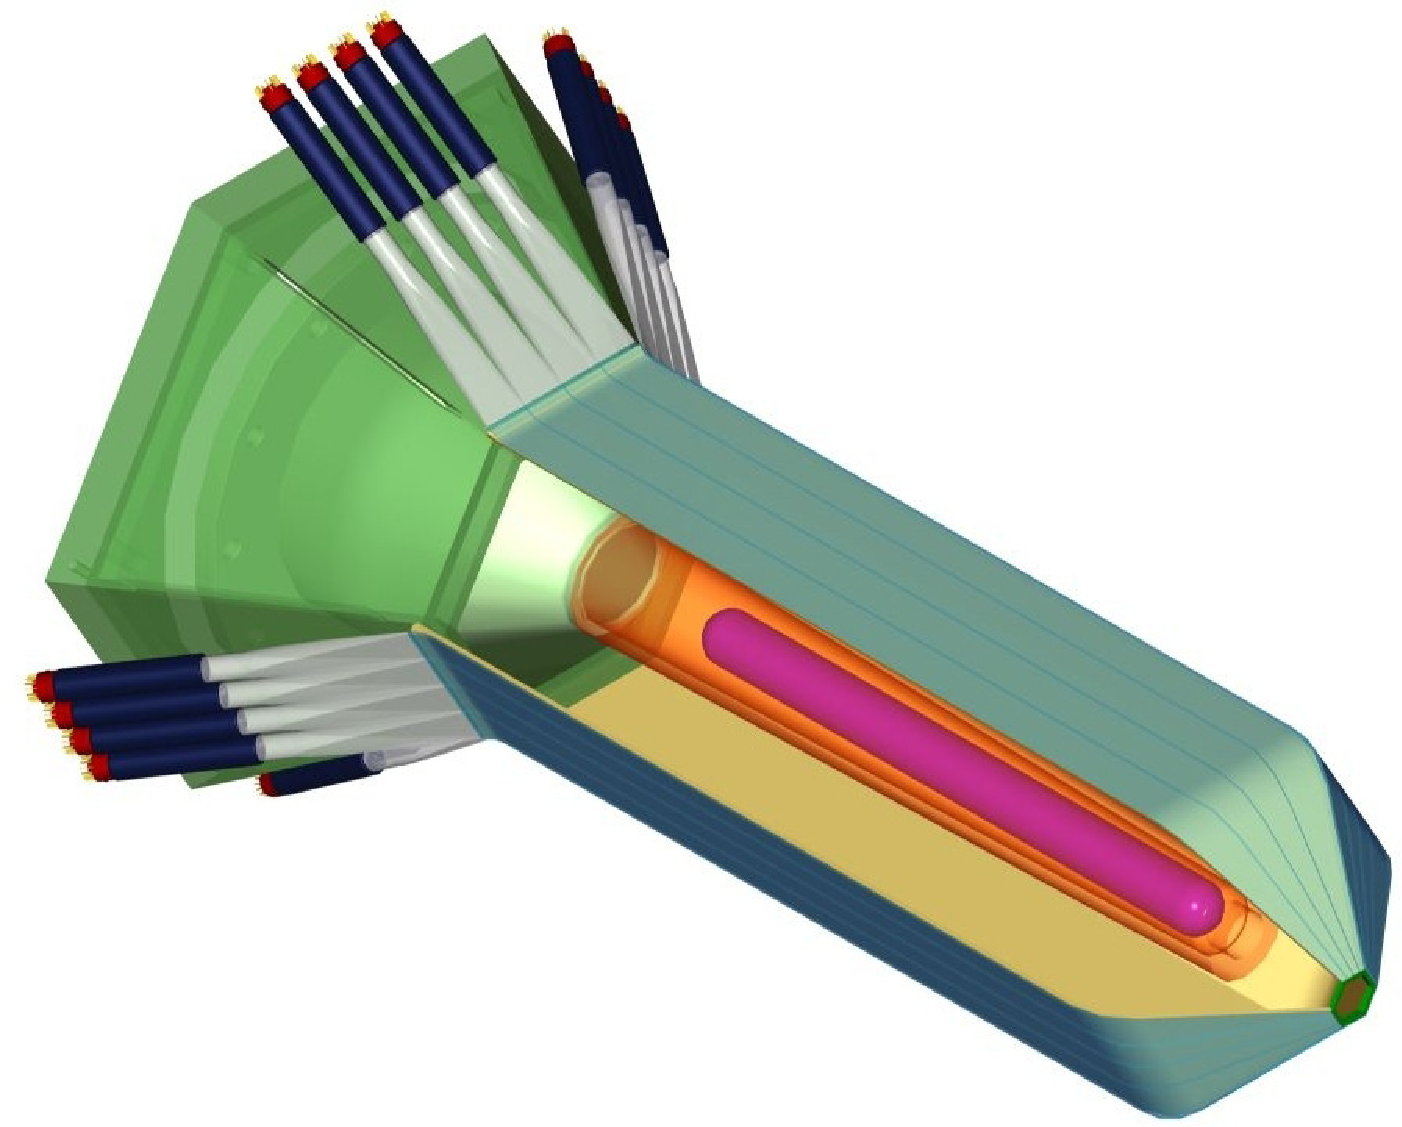
\includegraphics[width=0.8\figwidth,height=\qfigheight]{\grpath/hall-b/start_counter.pdf}
\caption[Start Counter Schematic]{\label{fig:clas.st}{\coloronline}Schematic of the start counter (\abbr{ST}) with the 40~cm long target cell (purple) at the center. The beam enters from the upper left of the figure.}
\end{center}\end{figure}

\begin{figure}[h!]\begin{center}
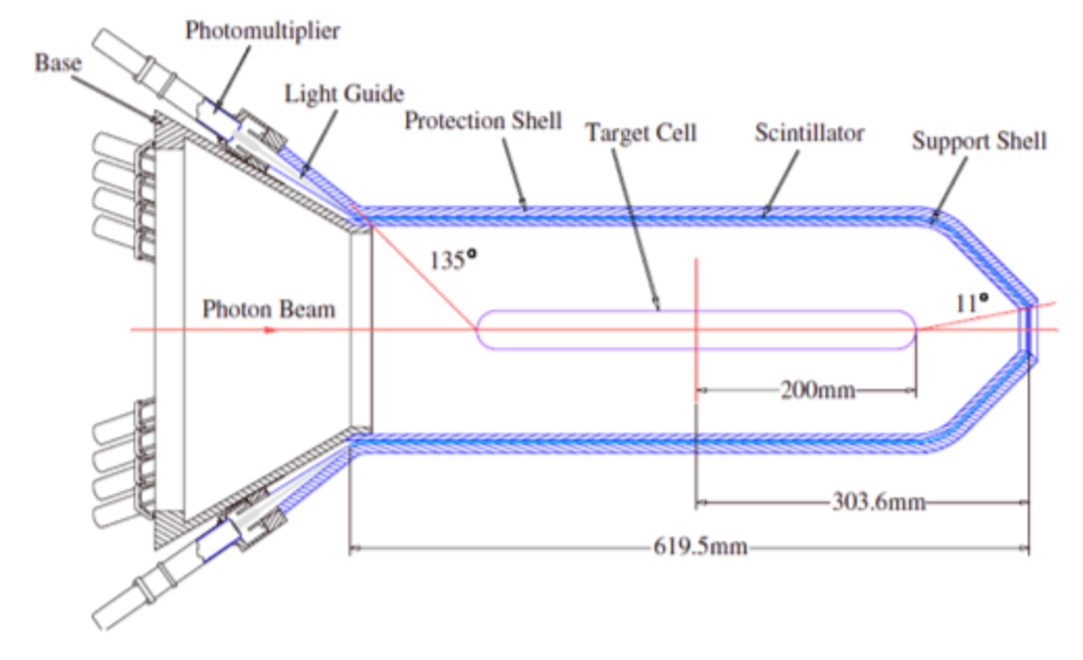
\includegraphics[width=0.8\figwidth,height=\qfigheight]{\grpath/hall-b/start_counter_wtarget.pdf}
\caption[Start Counter Schematic]{\label{fig:clas.stxsection}{\coloronline}Cross-section view of the start counter illustrating the labeled components and its angular coverage when at the center of \abbr{CLAS}.}
\end{center}\end{figure}

%\begin{figure}\begin{center}
%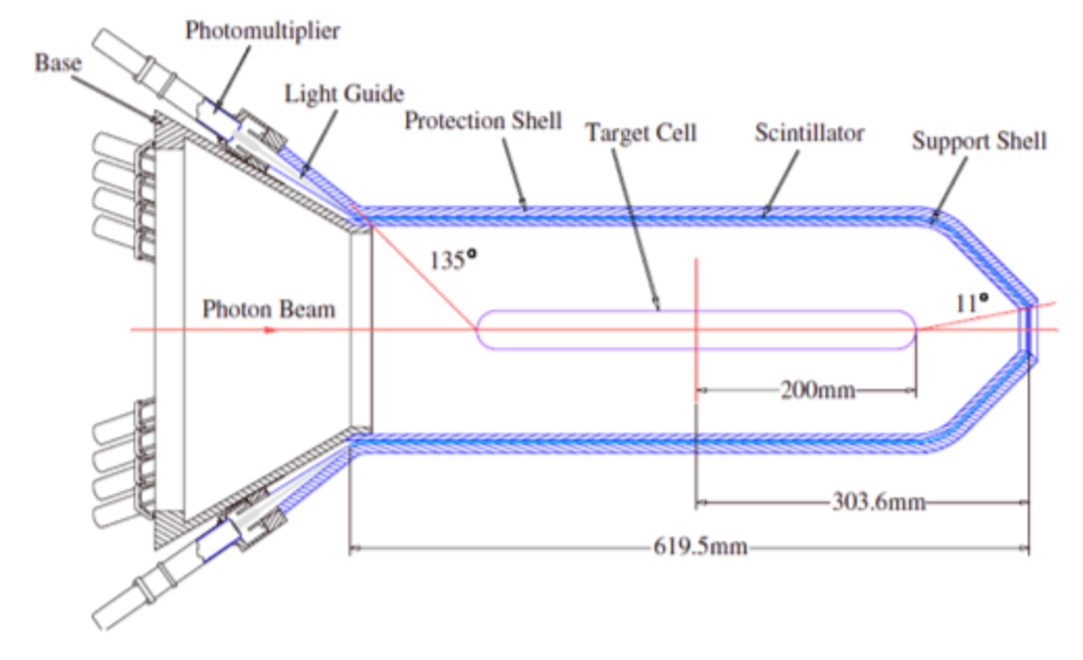
\includegraphics[width=0.8\figwidth,height=\qfigheight]{\grpath/hall-b/start_counter_wtarget.pdf}
%\caption[Cross_section view of \abbr{ST}]{\label{fig:clas.stxsection}{\coloronline}Cross-section view of the start counter illustrating the labeled components and its angular coverage when at the center of \abbr{CLAS}}
%\end{center}\end{figure}

%Put this in in a section Component coverage.
%\begin{figure}\begin{center}
%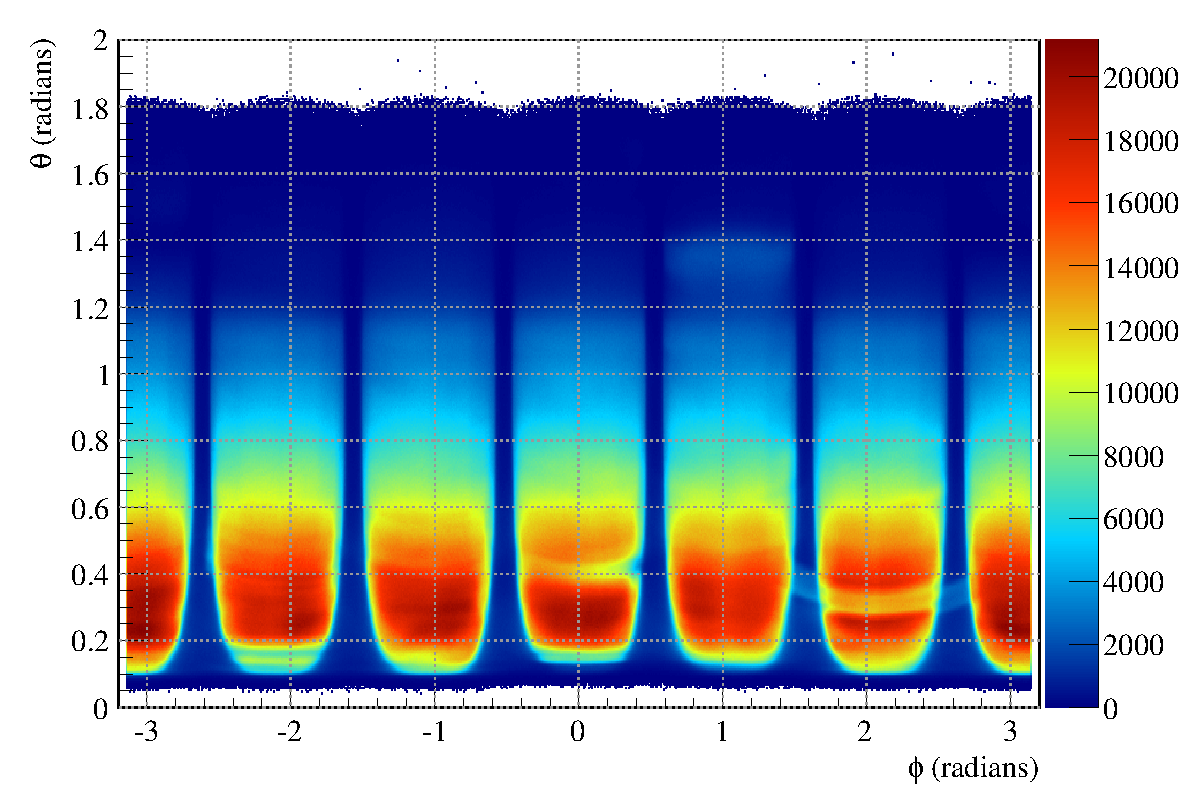
\includegraphics[width=\figwidth]{\grpath/reconstruction/coverage_st.pdf}
%\caption[Start Counter Angular Coverage]{\label{fig:clas.st.coverage}{\coloronline}Angular coverage in the lab frame of the tracks that had an associated start counter hit showing that the \abbr{ST} covered the entire \abbr{DC}/\abbr{TOF} acceptance region which is shown in Fig.~\ref{fig:clas.tof.coverage}.}
%\end{center}\end{figure}
\FloatBarrier
\subsection{Start Counter Efficiency Analysis}\label{sec:clas.st.eff}
There is an inefficiency of the start counter of 5~\% per track. This inefficiency was measured by using real data events as generated events and passing them through \abbr{CLAS}'s Monete-Carlo package(\abbr{GSIM}\label{abbr:gsim}). More information about this inefficiency will be dicussed in Sec.~\ref{sec:montecarlo}.

%It was observed that 20~\% of the events would fail in simulation, this will be discussed in Sec~\ref{sec:gsim.efficiency}. A portion of the failed events were based upon a failure to reconstruct the required banks for the start counter. This phenomena was investigated from the raw data and found to also be present in the processing of the data from raw to user file in the same manner as seen from Monte-Carlo. The blue-dashed line in Fig.~\ref{fig:classt.ineff} illustrates the start counter inefficiency that is dependent on the events reconstructed vertex. The inefficiency is due to the start counter reconstruction algorithm not being able to link the start counter hit to a track through time-based tracking. This track is not lost due to a reprocess of time-based tracking, linking the track to another particles start counter hit with the same 

%The inefficiency of the start counter is not a mechanical fault but rather the fault of the algorithm used to reconstruct a start counter hit. TO study this raw data events were processed event by event using the program DDD and \abbr{CLAS} event display (\abbr{ced}). Unknown of the cause, it  


\begin{figure}[h!]\begin{center}
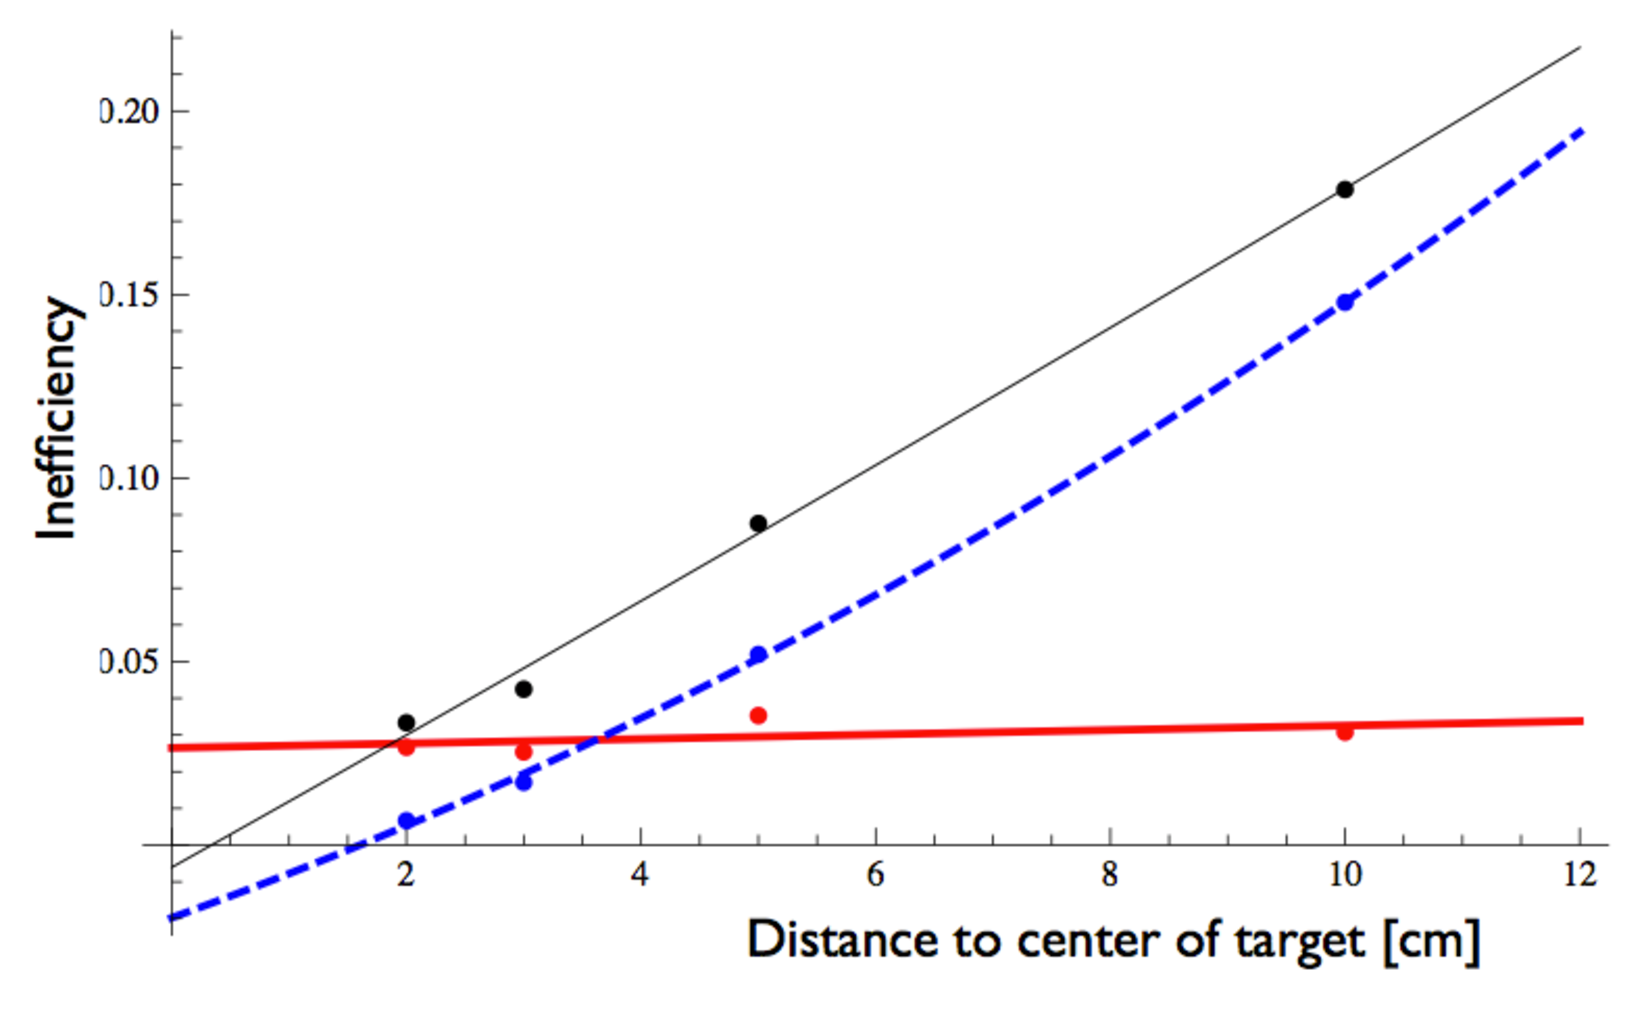
\includegraphics[width=0.8\figwidth,height=0.8\hfigheight]{\grpath/hall-b/st_issue_4_thesis.pdf}
\caption[Start Counter Inefficiency]{\label{fig:classt.ineff}{\coloronline}Plot showing the inefficiency of the start counter from data events, red-solid line is the inefficiency of reconstructing based solely on hit-based tracking, blue-dashed line is inefficiency of start counter, black-solid is combinatorial. }
\end{center}\end{figure}

%\begin{comment}
%
%\subsection{\label{sec:clas.st.eff}Efficiency Analysis}
%
%\todo{NOTE: I'm not sure if I want to keep this section. The numbers quoted are only from memory and are not reliable enough to put here at the moment.}
%
%About a year before \g12, we made some effort to understand the limiting factor on the \abbr{DAQ} rate for \abbr{CLAS}. At the time, it seemed that a start counter segmented in $\theta$ as well as $\phi$ might admit a higher beam current and therefore a higher physics event rate. Using phase-space Monte Carlo of three \emph{prong} events (p $\pi^+$ $\pi^-$) we were able to determine that two tracks will pass through the same \abbr{ST} paddle (in the current 24-paddle configuration) less than 5\% of the time. For topologies requiring four tracks, this increases to about 10\%. This only affects events on the trigger level, and since \g12 used a two-\emph{prong} trigger, the determination was that the 24-segment \abbr{ST} was sufficient. The tracks that use the same start counter hit in the data, since they enter the \abbr{ST} at about the same time, will not be lost during reconstruction.
%
%\begin{figure}\begin{center}
%%\includegraphics[width=0.8\figwidth]{\grpath/reconstruction/start_counter_eff.pdf}
%\caption[Start Counter Efficiency]{\label{fig:clas.st.eff}\todo{This plot must be recreated} Percentage of the track pairs that enter the same \abbr{ST} paddle for topologies increasing in number of particles. The trigger used for \g12 had a two-\emph{prong} configuration and therefore the number events lost at the trigger level was $<1\%$.}
%\end{center}\end{figure}
%
%\end{comment}
